%%%%%%%%%%%%
%
% $Autor: Wings $
% $Datum: 2019-03-05 08:03:15Z $
% $Pfad: LEDPower $
% $Version: 4250 $
% !TeX spellcheck = en_GB/de_DE
% !TeX encoding = utf8
% !TeX root = filename 
% !TeX TXS-program:bibliography = txs:///biber
%
%%%%%%%%%%%%


%todo citations
%todo create tikz pictures
%todo test the code

\chapter{Power LED}\index{LED!Power LED}

Arduino boards have a power LED on board. Normally, the power LED indicates the status of the board.

\section{General Information}

The power LED on an Arduino board is a small, usually red or green, \ac{led} that indicates whether the board is receiving power.
It is typically located near the USB connector on the board. When the board is powered on, the \ac{led} will illuminate.
The specific color and behavior of the power LED may vary depending on the Arduino board model.
For example, on the Arduino Uno, the power LED is red and illuminates steadily when the board is powered on.
On the Arduino Nano, the power LED is green and blinks slowly when the board is powered on.
The power LED is a helpful visual indicator that can be used to troubleshoot power supply issues.
If the power LED is not illuminated, it means that the board is not receiving power.
This could be due to a number of reasons, such as a loose USB connection, a damaged power supply, or a problem with the board itself.
By checking the power LED, you can quickly identify and resolve power supply problems with your Arduino board.

\Mynote{cite books}

\section{Specific Sensor}

While labeled as a power LED, the single green \ac{led} on the Nano 33 BLE Sense isn't solely for power indication. It has multi-functionality depending on board state and user code interaction. During typical operation, it lights steadily green when powered, similar to other Arduino models.
However, it flashes rapidly during serial communication and bootloader mode.
Notably, when user code enters deep sleep mode, the \ac{led} turns off entirely for power saving. This includes power status, communication activity, and sleep mode activation.
Understanding these \ac{led} behaviors can aid in troubleshooting and code debugging.
The green power LED's primary function remains indicating power and basic board states.


\Mynote{cite Arduino}


\begin{center}    
  \begin{tikzpicture}
      
   
    \node at (0,0) (Board) {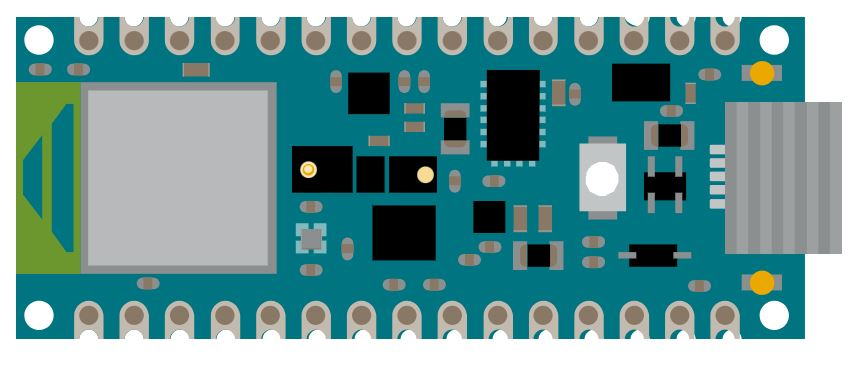
\includegraphics{Arduino/Nano33BLE/Nano33BLESense}};

    \fill[gray, opacity=0.7] (-6,-2.4) rectangle (6,2.4);
    
    \coordinate (A) at (4,-1.6);
    \coordinate (B) at (4.9,-1.1);    
    \begin{scope}
      \clip (A) rectangle (B);

      \node at (0,0) (Board) {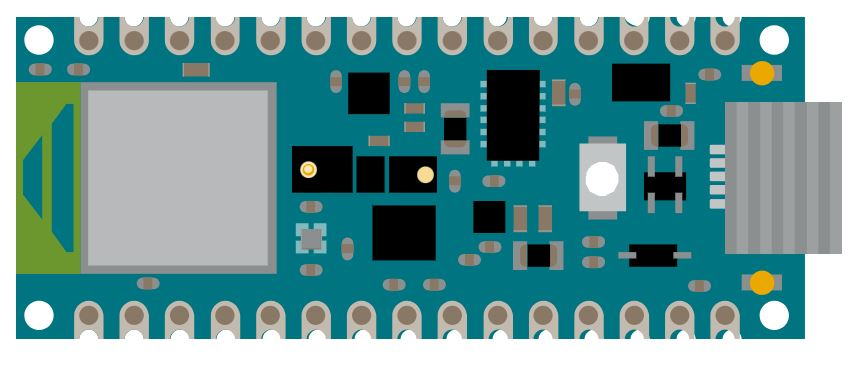
\includegraphics{Arduino/Nano33BLE/Nano33BLESense}};

    \end{scope}
    \draw[yellow,line width=2pt] (A)  rectangle (B);
  \end{tikzpicture}    

  \captionof{figure}{Arduino Nano 33 BLE Sense's Power LED}  
\end{center}

\Mynote{tikz picture with power LED}
    

\section{Specification}

The power LED is a green \ac{led} and connected to pin 25.\index{Pin!Pin 25} The brightness can be controlled via \ac{pwm}.

\begin{description}
    \item [Power LED:] \PYTHON{LED\_PWR =  25u}
\end{description}

Power LED is active-high and connected to pin 25.

The power LED can also be controlled programmatically by setting the pin to \PYTHON{HIGH} or \PYTHON{LOW}. 


\Mynote{cite data sheet, power consumption?}

The pin must be defined as an output in the function \PYTHON{setup} by setting \PYTHON{pinMode (LED\_PWR, OUTPUT)}, otherwise the \ac{led} cannot be switched on.

\medskip 


The pin 25 can also be used otherwise. Then the \ac{led} is just switched on if the board is connected to a power source. \Mynote{to be tested!}

\Mynote{What happen if there is another \ac{led} at the pin? Both in use?}

%\section{Calibration}
%
%cite method

\section{Simple Code}

In the sketch \ref{Nano:PowerLEDTest}, a variable is connected to pin 25.\index{Pin!Pin 25} The pin 25 is defined as an output in the function \PYTHON{setup}. In the function \PYTHON{loop}, the \ac{led} is switched on for 1 second and switched off for 1 second so that the \ac{led} flashes accordingly.



{
  \captionof{code}{Simple sketch to control the power LED}\label{Nano:PowerLEDTest}
  \ArduinoExternal{}{../Code/Nano33BLESense/Test/TestLEDPower.ino}
}

\bigskip

This is just a simple example. The variable \PYTHON{LED\_PWR} is already defined, so the assignment is not necessary. The command \PYTHON{delay} should be avoided in an Arduino sketch. Instead, variables of the type \PYTHON{elapsedMillis} should be used.

\Mynote{Arduino Referenz \url{https://github.com/pfeerick/elapsedMillis/wiki}}


\section{Tests}

\subsection{Simple Function Test}

The simplest test is the flashing of the \ac{led} at 2 Hz.

{
  \captionof{code}{Simple sketch to test the power LED}\label{Nano:PowerLEDTest}
  \ArduinoExternal{}{../Code/Nano33BLESense/Test/TestLEDPower.ino}
}


\subsection{Test all Functions}

The brightness of the power LED can be controlled. This is demonstrated in the example sketch \ref{Nano:PowerLEDTestPWM}.

Using the pulse width modulation, the brightness is gradually increased to the maximum value and then gradually reduced to 0 again.




{
    \captionof{code}{Simple sketch to check the battery state using the power LED}\label{Nano:PowerLEDTestPWM}
    \ArduinoExternal{}{../Code/Nano33BLESense/Test/TestLEDPowerBrightness.ino}
}


\section{Simple Application}


There are different situations where it might be useful to program the power LED of the Arduino Nano. For example, you could use it to:

\begin{itemize}
    \item Indicate the status of the board, such as whether it is connected to a power source, a computer, or a sensor.
    \item  Display the battery level of the board, by changing the brightness or color of the power \ac{led}.
    \item Create a visual alarm or notification, by making the power LED blink or flash in a certain pattern.
\end{itemize}

\bigskip

A simple application is to check the condition of the battery. The sktech \ref{Nano:PowerLEDTestBattery} demonstrates, if the voltage drops too low, the power LED flashes.

{
    \captionof{code}{Simple sketch to check the battery state using the power LED}\label{Nano:PowerLEDTestBattery}
    \ArduinoExternal{}{../Code/Nano33BLESense/Test/TestLEDPowerBattery.ino}
}


\section{Further Readings}


\Mynote{citations}

